\chapter{Introduction}
This chapter contains a brief introduction to Australian Indigenous seasonal calendars,
explains the focus, novelty, and delimitations of this research,
and lays out the structure of the thesis.

~\\

Also needs to lay out the wider story of why seasons are important,
which becomes a narrative thread throughout the thesis.
This should answer the `why bother' question, and justify the research.


\section{Indigenous Seasons and Ecological Knowledge}
% - One paragraph on the global-scale reason to care about the topic
% - Lay out how Indigenous seasons are defined (inc. international, contrast)
% - draw link to ecological knowledge
% - Explain shortcomings in existing research


This thesis investigates and characterises an Indigenous seasonal calendar.
I combine Indigenous knowledge with Western climate science to characterise
local seasonality in NE Arnhem Land (see \autoref{fig:arnhem-map}),
as described by a Yolngu seasonal calendar I construct based on
interviews and supported by literature.


Where Australia's formally recognised seasons are defined by Gregorian date -
e.g. December 1 is by definition the first day of Summer - Indigenous seasons
are defined by weather and ecological events.
%
This more closely matches intuitions about seasons as annually recurring
periods marked by weather - most commonly temperature, which tends to
follow sunlight intensity - than a date-based approach, though Indigenous
seasons are more nuanced than ``hot == summer, cold == winter''.

Like the observation-based approach used in some Nordic nations, where
seasons are defined by persistent temperature change (REF),
Indigenous Australian seasons are recognised after the fact and vary
between years depending on the behaviour of their indicators.


A Yolngu seasonal calendar was chosen as the case study for this thesis
as personal relationships in the region facilitated qualitative research,
and the emphasis on meteorological indicators allows quantification based
on the observational weather record.
    


~\\
~\\
Section beyond this point is DRAFT NOTES ONLY


Highly localised.
Yolngu calendars of North-East Arnhem Land divide the year into
six seasons based on prevailing wind, rainfall, temperature,
and a variety of other factors.

Derivation of the seasonal calendar from current conditions,
along with the impossibility of applying the European seasonal calendar
to the tropical seasonality, make Yolngu seasons an excellent case study.

See \citet{menzel2006} re modern scientific use of ecological changes
as indicators of seasonal onset or climate change.



Indigenous knowledge is recognised and valued in an increasing variety
of contexts \citep[eg.][]{petheram2010,cochran2015,berkes2012} –
but integration with the physical sciences is still relatively rare and ad-hoc.
%
I argue that such synthesis provides a crucial long-term perspective on
anthropogenic environmental change, and demonstrate that such synthesis
can produce novel results for both scientific and indigenous stakeholders.

Ecological knowledge is embedded in calendars.



\section{Delimitations and novelty}
% May want to present novelty, then delimitations...

NEEDS PARA ON DELIMITATIONS - see and work from mid-course review feedback to inform this.

~\\

Existing research on indigenous calendars has focussed on the social or ecological aspects,
documenting indigenous knowledge – see eg \textit{Man of All Seasons} \citep{davis1989},
the Indigenous Weather Knowledge project \citet{BOM-iwk},
or CSIRO’s Tropical Rivers and Coastal Knowledge (TRaCK) program \citep{CSIROcals,oconnor2010}.

There is however a paucity of research which treats indigenous knowledge
as a \emph{framework for} research, instead of an \emph{object of} research.

This trend manifests as a gap in the literature (see \autoref{ch:lit-review}),
despite the novely and potential value of combining Indigenous seasonal knowledge
with quantitative climate science.

PARA ON LIT SEARCH STRATEGY

None of the participants I interviewed were aware of attempts to quantify indigenous seasons,
and several made spontaneous comments as to the novelty of this approach.





\section{Structure of the Thesis}

This document is structured with a variation of the standard format for scientific reports,
where the body chapters for a literature review, methods, and results
have been organised by topic rather than content.

The aim of this format is present the four logical stages of my research
in ordered and reasonably self-contained chapters.
It also reflects the overarching methodology of distinct steps that are
later extended.  The academic and local context provides direction and focus
for the qualitative research.  In turn, the qualitative data and context
allows construction of a bridge to quantitative data and methods.


\paragraph{Context:}
\autoref{ch:context}, \textit{\nameref{ch:context}} contextualises the research.
It covers the basic context of the research,
regarding the location and past studies of the Yolngu calendar;
finds a gap in the literature and surveys relevant fields;
and lays out the overarching methodology of and strategy for this research.

Note that while the overarching methodology and general review of the relevant literature
are contained in this section, each of the body chapters describes the applicable methods
and references more specific literature as appropriate.


\paragraph{Qualitative:}
\autoref{ch:seasons}, \textit{\nameref{ch:seasons}} focusses on the qualitative research component.
It discusses interview methods, considerations for indigenous knowledge, and integration with literature.
The primary results are a reflection on process and outcomes,
and a qualitative description of Yolngu seasons.


\paragraph{Bridging:}
\autoref{ch:quantify}, \textit{\nameref{ch:quantify}} shows the creation of a quantified Yolngu calendar.


\paragraph{Quantitative:}
\autoref{ch:analysis}, \textit{\nameref{ch:analysis}} shows the analysis of the quantified calendar.



\section{Context and importance of this research}
\label{ch:context}
This chapter covers the basic context of the research,
regarding the location and past studies of the Yolngu calendar,
and lays out the overarching methodology of and strategy for this research.


\begin{figure}[h]
    \centering
    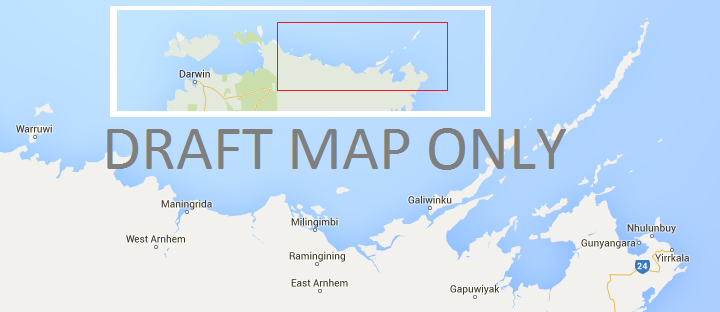
\includegraphics[width=\textwidth]{mapdraft.png}
    \caption[Map showing the study area, NE Arnhem Land]{
        Map showing the study area, NE Arnhem Land.
        Analysis in \autoref{ch:quantify} uses weather observations from several of the towns shown.
        }
    \label{fig:arnhem-map}
\end{figure}


This study focusses on North-East Arnhem Land, particularly Elcho Island
and the town of Galiwinku.  Figure~\ref{fig:arnhem-map} shows the study area.
Qualitative seasonality is described for Galiwinku and Milingimbi;
quantitative weather observations are from Waruwi, Maningrida, Milingimbi,
Galiwinku, and Nhulunbuy.

These sites are all in Yolngu country, in the Anrhem Coast bioregion \citep{ens2014}.
The landscape is dominated by tropical woodland, from mangroves on the coastline 
through dense forest to more open woody grasslands further inland.

Yolngu have a tradition of engagement across cultures, including
the Macassan trade with Indonesia in the 1700s and engagement with Methodist
missionaries throughout the 1900s.

% RELEVANCE UNCLEAR; REVISE BARK PETIION REFERENCES
The Yirrkala Bark Petition (\autoref{fig:bark-petition}) marks a crucial
point in the Australian land rights movement, recognised by indigenous and
non-indigenous people alike.  It is also prone to misinterpretation by those
who see a document in two languages with a decorative border: the border
is the most important part!  (see caption, expand this section)


\begin{wrapfigure}{R}{0.5\textwidth}
    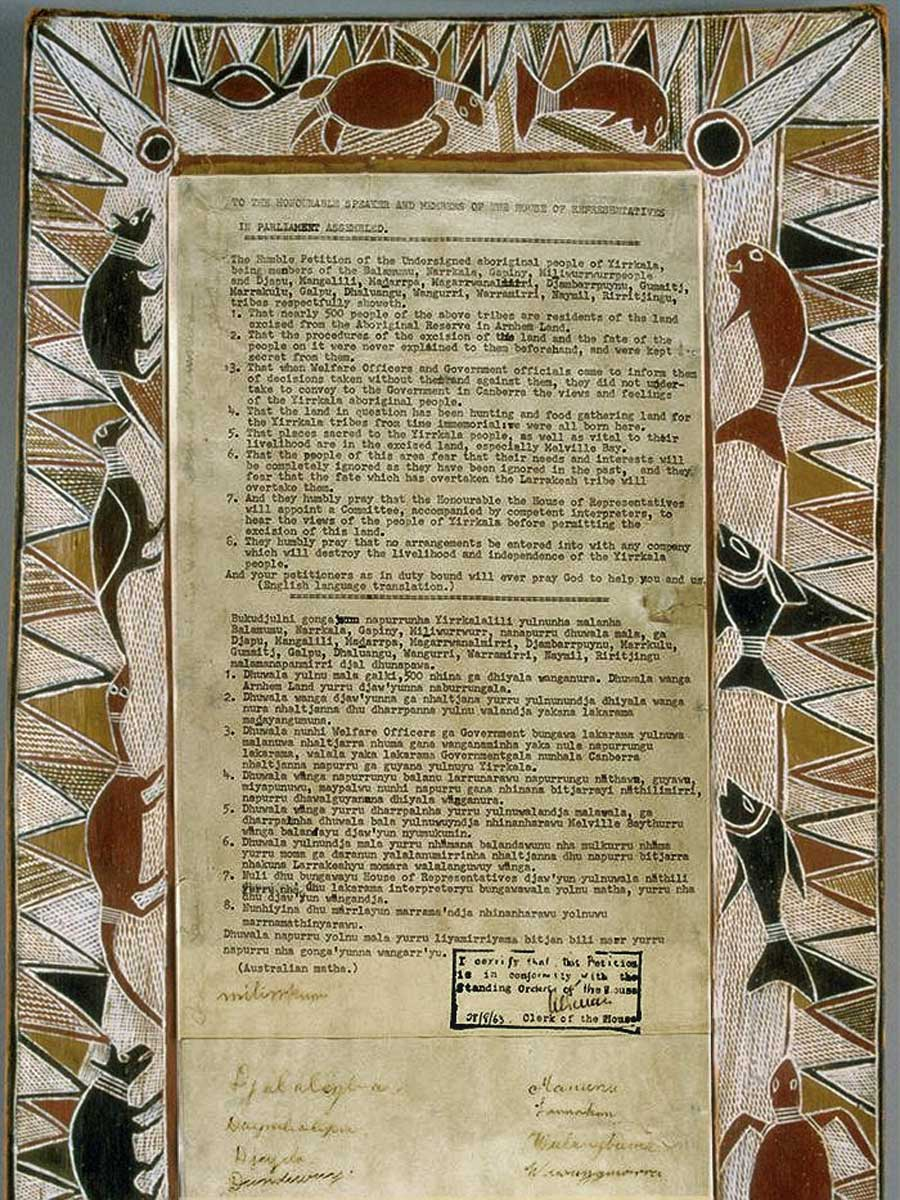
\includegraphics[width=\linewidth]{bark-petition.jpg}
    \caption[The Yirrkala Bark Petition]{
        The Yirrkala Bark Petition, 1963.
        The Bark Petition concerns the bauxite mining lease granted at Nhulunbuy
        without consultation with Yolngu, and helped kick-start the Australian
        land rights movement.

        The petition is presented in three ways: text in English,
        text in Yolngu Matha, and in the border.
        This painting is not a decoration; it is a reproduction of
        the title deeds to the ancestoral estates of the signatories -
        and the most important part of the document.
        }
    \label{fig:bark-petition}
\end{wrapfigure}


In a letter inviting collaboration on this research (see \autoref{sec:ethics}),
a senior Yonlgu man explained that:

\blockquote{
    For Yolngu (the people of North Eastern Arnhem Land) it is the Liyagadhaman
    who carry within them the wisdom and knowledge of these matters.
    It is right that in this research you have approached me to talk about these
    things. I can also introduce you to others who have this knowledge.  ...

    Yolngu have made careful observation of the ways of nature and the seasons
    over the millennia and have passed on that knowledge down the generations.
    We know the changes that are taking place in the seasons and I am willing
    to talk with you about what I have seen happening around me.
}




The BOM describes the 
climate as ``hot and humid'', with daytime temperatures between 25 and 40 
degrees year-round.  Rainfall and humidity are dominated by monsoon 
seasonality, and the seasons are commonly described by non-indigenous residents 
as “the Wet” and “the Dry” – though after a few years many also recognise “the 
Buildup” of pre-wet humidity \citep{willmett2009}.

The key meteorological determinants of seasonality are temperature (especially 
night-time), rainfall, humidity, and wind strength and direction.  The annual 
cycle is driven primarily by the Indian Ocean monsoon.  The seasonal effect of 
temperature is felt most strongly at night, as daytime temperatures are very 
consistent and the latent heat of available water has a strong effect.

However, wet/dry/buildup misses important nuance in the seasonality of the 
area.  \autoref{fig:yolngu-seasons} shows one summary of Yolngu seasonality,
with significantly more seasons.  \citet{woodward2012b} notes
\blockquote{
    four factors that interconnect within each of the seasonal
    knowledge systems; a focus on resource use, knowledge of complex
    ecological indicators to facilitate resource collection,
    knowledge of meteorological phenomena and a strong
    metaphysical/spiritual understanding.
}

